\documentclass[ignorenonframetext,]{beamer}
\setbeamertemplate{caption}[numbered]
\setbeamertemplate{caption label separator}{: }
\setbeamercolor{caption name}{fg=normal text.fg}
\beamertemplatenavigationsymbolsempty
\usepackage{lmodern}
\usepackage{amssymb,amsmath}
\usepackage{ifxetex,ifluatex}
\usepackage{fixltx2e} % provides \textsubscript
\ifnum 0\ifxetex 1\fi\ifluatex 1\fi=0 % if pdftex
\usepackage[T1]{fontenc}
\usepackage[utf8]{inputenc}
\else % if luatex or xelatex
\ifxetex
\usepackage{mathspec}
\else
\usepackage{fontspec}
\fi
\defaultfontfeatures{Ligatures=TeX,Scale=MatchLowercase}
\fi
\usetheme{AnnArbor}
\usecolortheme{dolphin}
\usefonttheme{professionalfonts}
% use upquote if available, for straight quotes in verbatim environments
\IfFileExists{upquote.sty}{\usepackage{upquote}}{}
% use microtype if available
\IfFileExists{microtype.sty}{%
\usepackage{microtype}
\UseMicrotypeSet[protrusion]{basicmath} % disable protrusion for tt fonts
}{}
\newif\ifbibliography

% Prevent slide breaks in the middle of a paragraph:
\widowpenalties 1 10000
\raggedbottom

\AtBeginPart{
\let\insertpartnumber\relax
\let\partname\relax
\frame{\partpage}
}
\AtBeginSection{
\ifbibliography
\else
\let\insertsectionnumber\relax
\let\sectionname\relax
\frame{\sectionpage}
\fi
}
\AtBeginSubsection{
\let\insertsubsectionnumber\relax
\let\subsectionname\relax
\frame{\subsectionpage}
}

\setlength{\parindent}{0pt}
\setlength{\parskip}{6pt plus 2pt minus 1pt}
\setlength{\emergencystretch}{3em}  % prevent overfull lines
\providecommand{\tightlist}{%
\setlength{\itemsep}{0pt}\setlength{\parskip}{0pt}}
\setcounter{secnumdepth}{0}


% \pgfdeclareimage[width=1cm]{logo}{}
%\logo{\pgfuseimage{logo}}

\institute{UVa/UCI}
\definecolor{links}{RGB}{42, 27, 129}
\definecolor{mypink2}{RGB}{219, 48, 122}
%\hypersetup{colorlinks,linkcolor=links,urlcolor=mypink2}
\usefonttheme{professionalfonts}

% \setbeamerfont{note page}{family*=pplx,size=\footnotesize} % Palatino for notes

\setbeamerfont{subtitle}{size=\small}

\definecolor{uciblue}{RGB}{0,100,164}
\definecolor{ucilibraryorange}{RGB}{255,210,0}
\definecolor{ucicream}{RGB}{241,229,199}
\definecolor{ucilightblue}{RGB}{163,220,230}

\setbeamercolor{block body}{bg=green,fg=green}
\setbeamercolor{block body alerted}{bg=green,fg=green}
\setbeamercolor{block body example}{bg=green,fg=green}

\setbeamercolor{caption name}{fg=uciblue}

\setbeamercolor{headline}{fg=ucicream,bg=ucicream}
\setbeamercolor{section}{fg=ucilibraryorange,bg=uciblue}
\setbeamercolor{frametitle}{fg=ucilibraryorange,bg=uciblue}
\setbeamercolor{palette primary}{bg=ucilibraryorange,fg=uciblue}
\setbeamercolor{palette secondary}{bg=uciblue,fg=uciblue}
\setbeamercolor{palette tertiary}{bg=ucilibraryorange,fg=uciblue}
\setbeamercolor{palette quarternary}{fg=ucilibraryorange,bg=uciblue}
\setbeamercolor{palette sidebar primary}{bg=ucilibraryorange,fg=uciblue}
\setbeamercolor{palette sidebar secondary}{fg=uciblue,bg=uciblue}
\setbeamercolor{palette sidebar tertiary}{fg=ucilibraryorange,bg=uciblue}
\setbeamercolor{palette sidebar quarternary}{fg=ucilibraryorange,bg=uciblue}
\setbeamercolor{structure}{bg=uciblue}



\useinnertheme{rectangles}

% \titlegraphic{\vspace{-7.5mm}\includegraphics[width=0.45\paperwidth]{../Figures/antsCollaborators2.png}}

\title{The ANTs longitudinal cortical thickness pipeline}
\author{N. Tustison et al.}
\date{}

\begin{document}
\frame{\titlepage}

\section{Longitudinal cortical structural changes from
MRI}\label{longitudinal-cortical-structural-changes-from-mri}

\begin{frame}{FreeSurfer longitudinal pipeline}

\centering
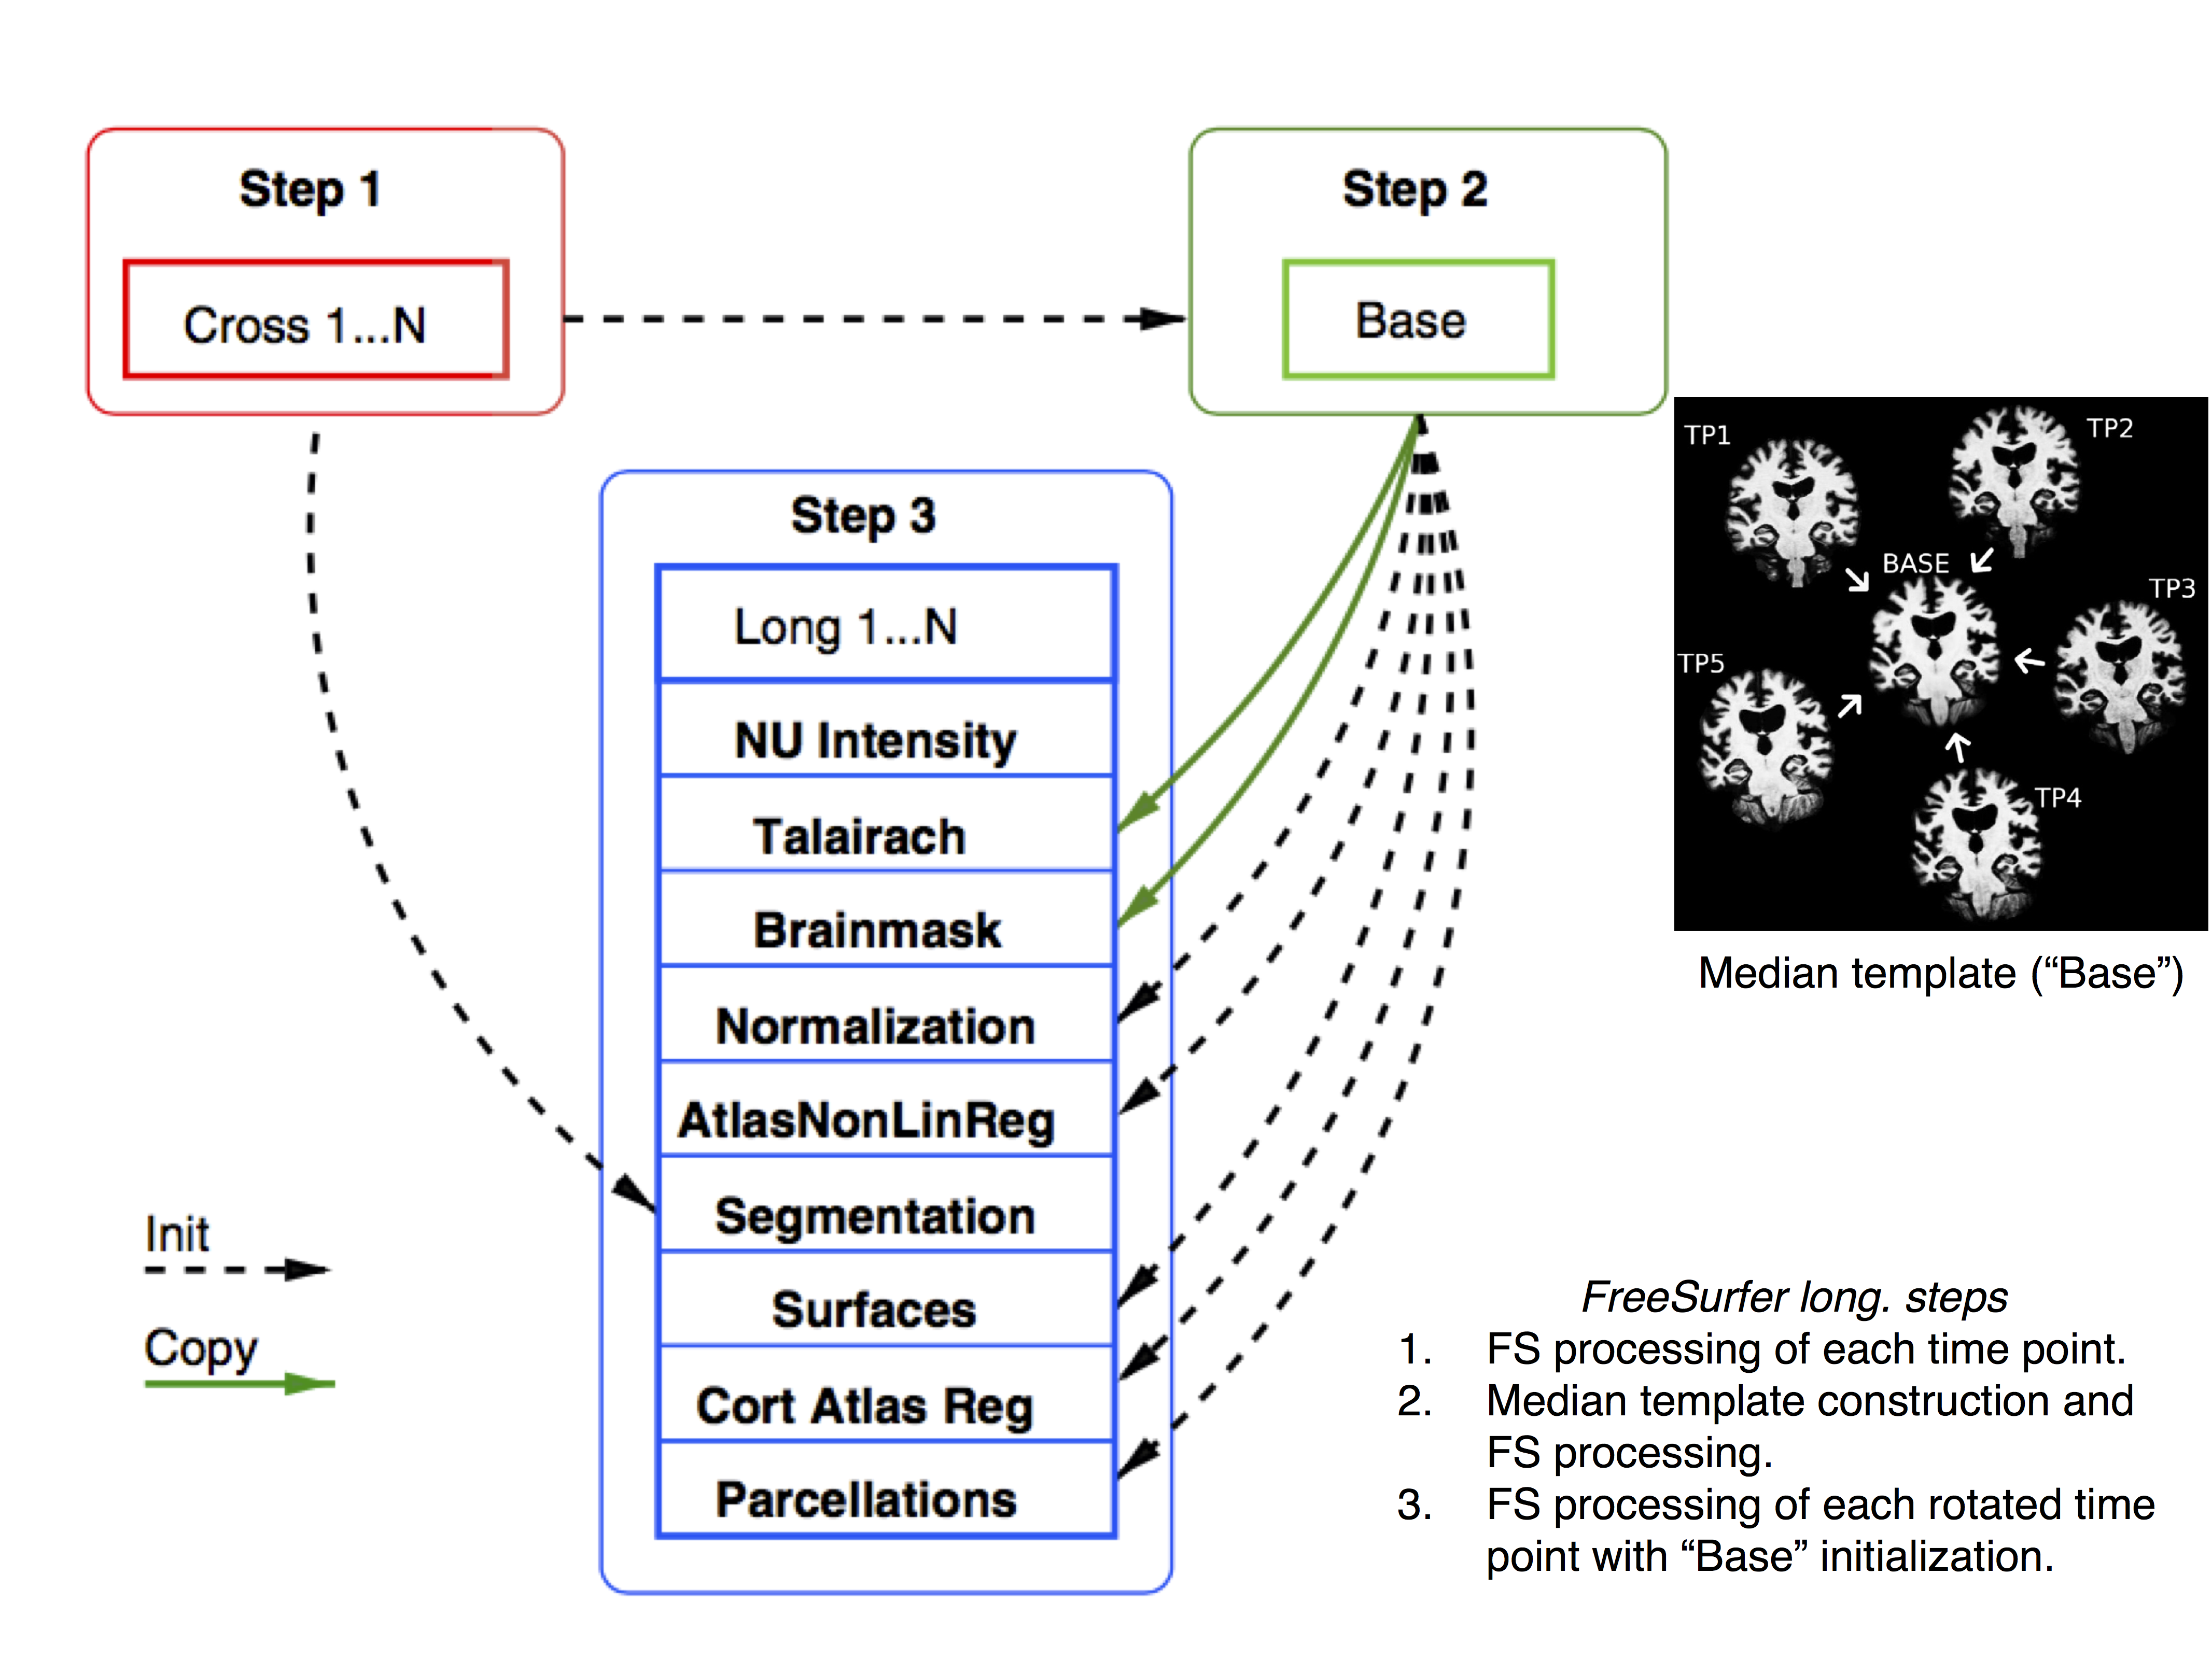
\includegraphics[width=0.85 \textwidth]{../Figures/FreeSurferLong.png}

\end{frame}

\begin{frame}{ANTs longitudinal pipeline}

\centering
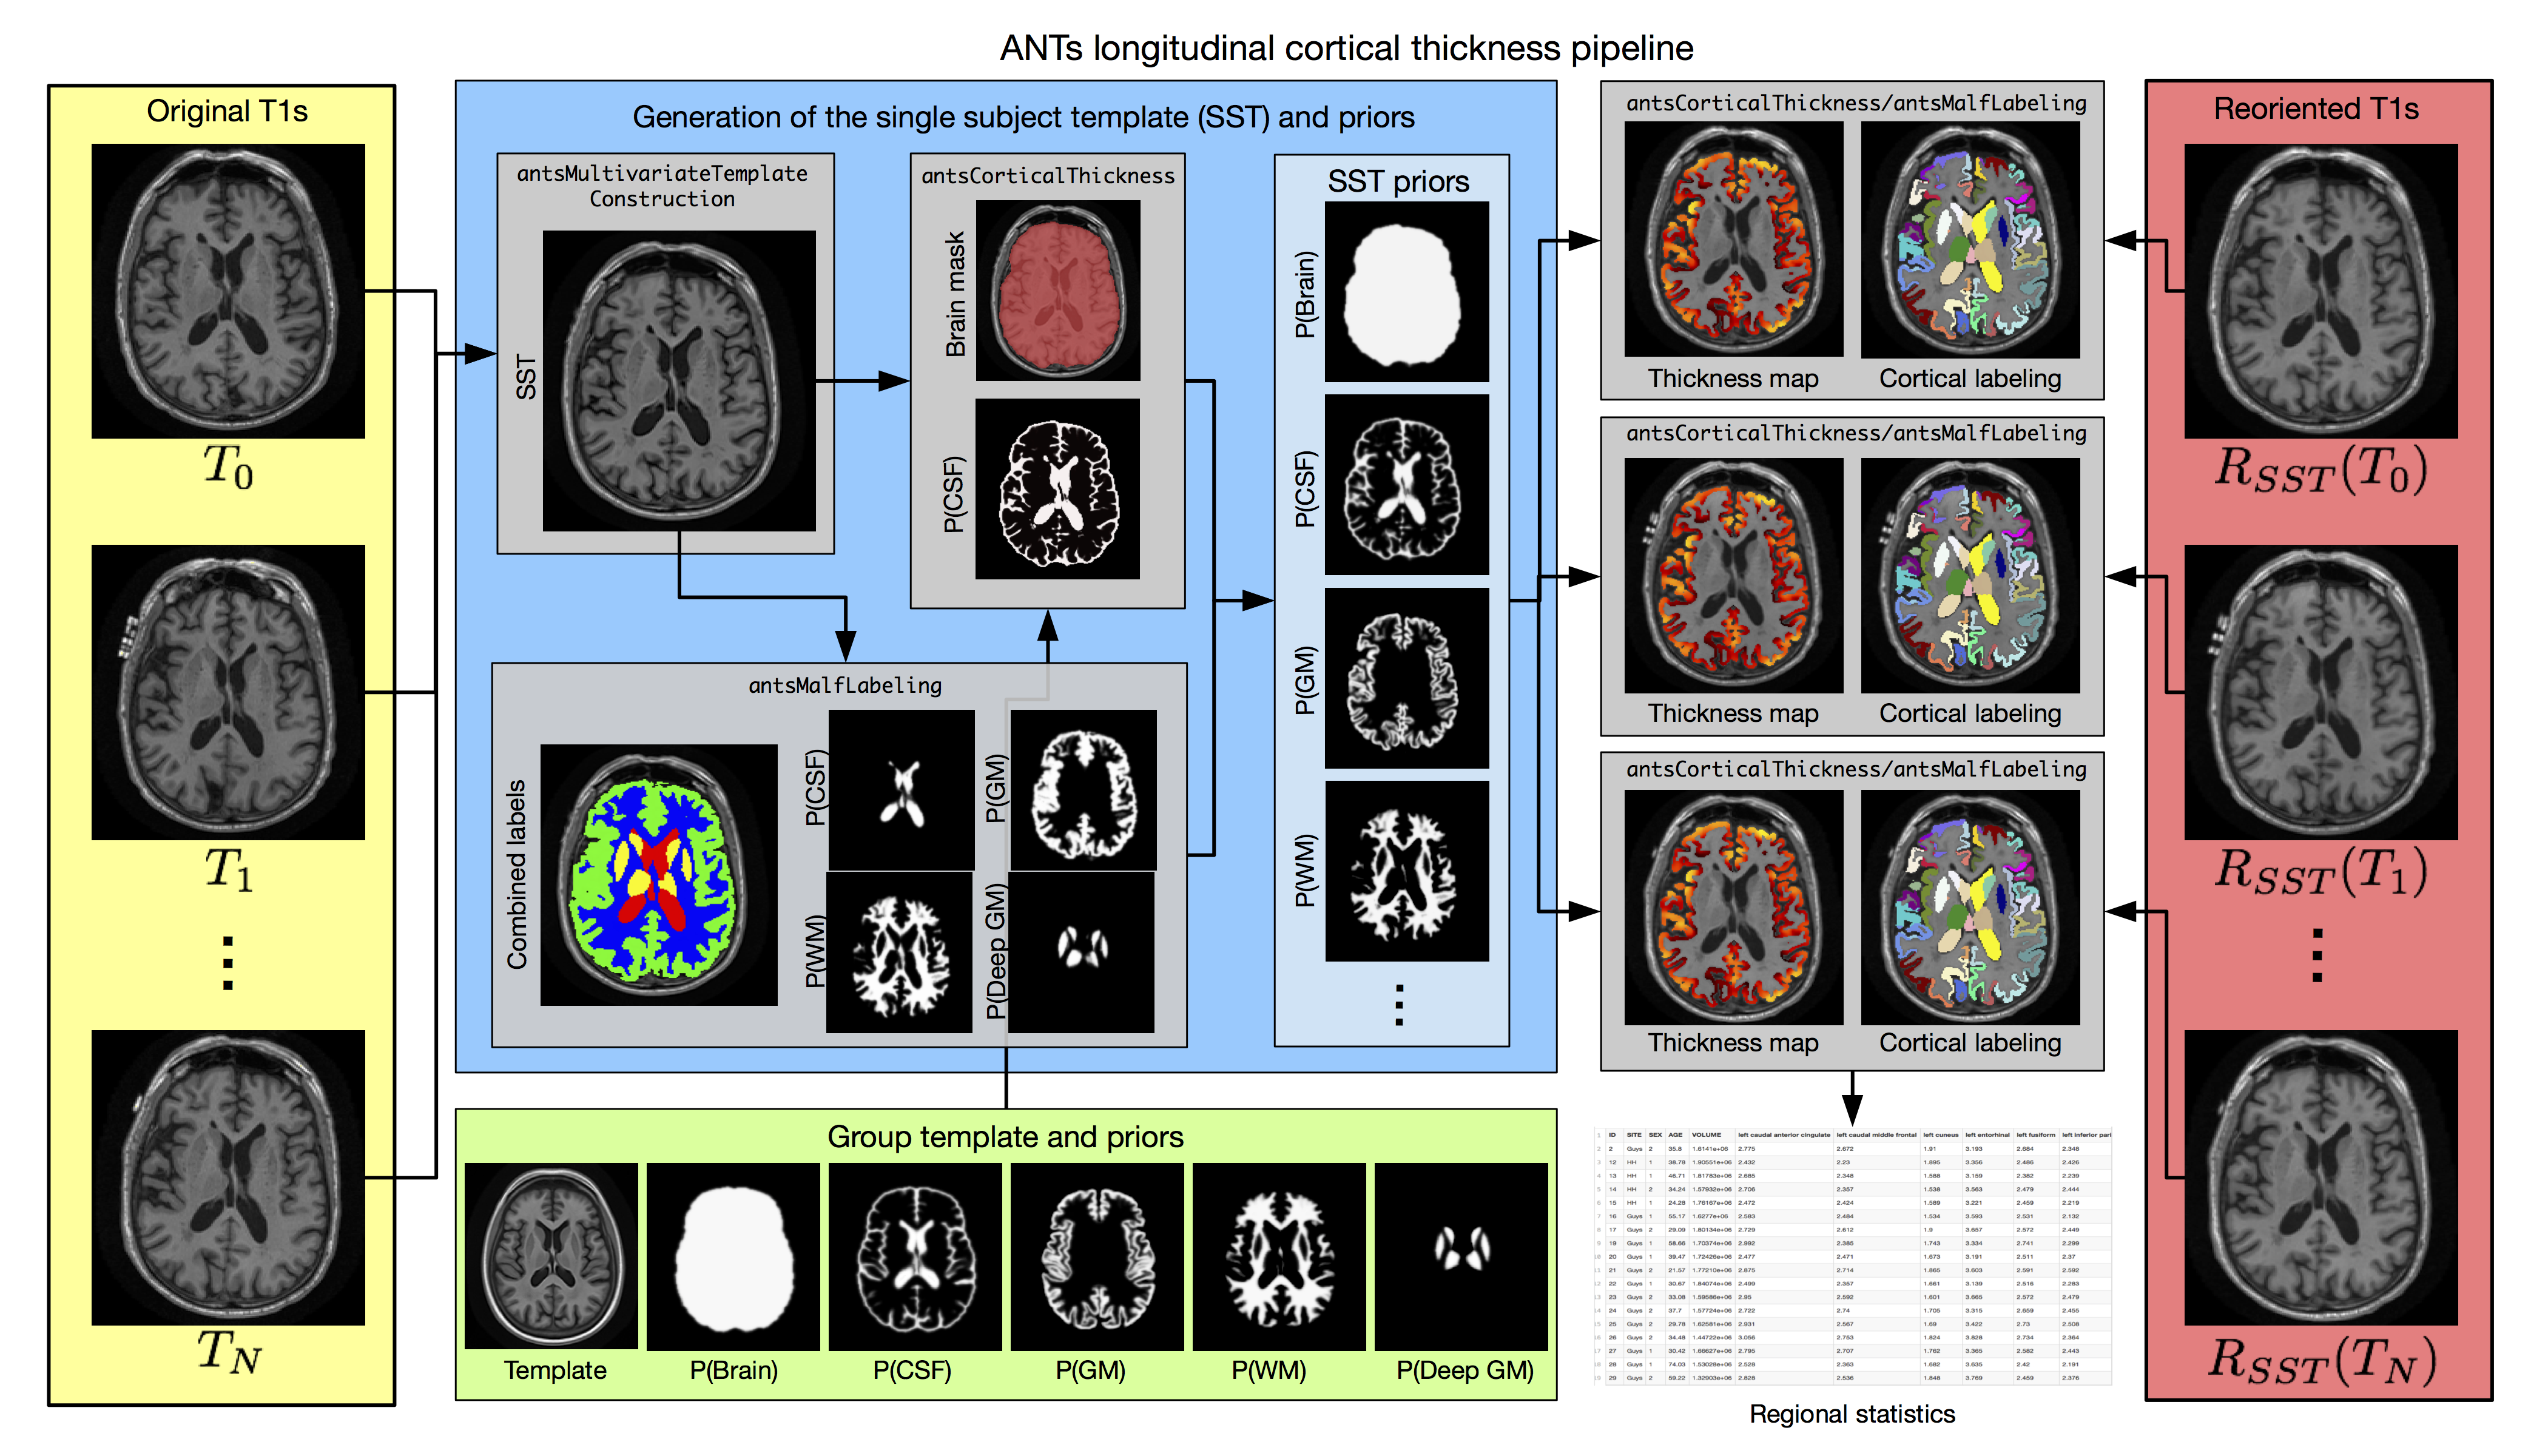
\includegraphics[width=0.99 \textwidth]{../Figures/longitudinalPipeline.png}

\end{frame}

\begin{frame}{Cross-sectional comparison}

\centering
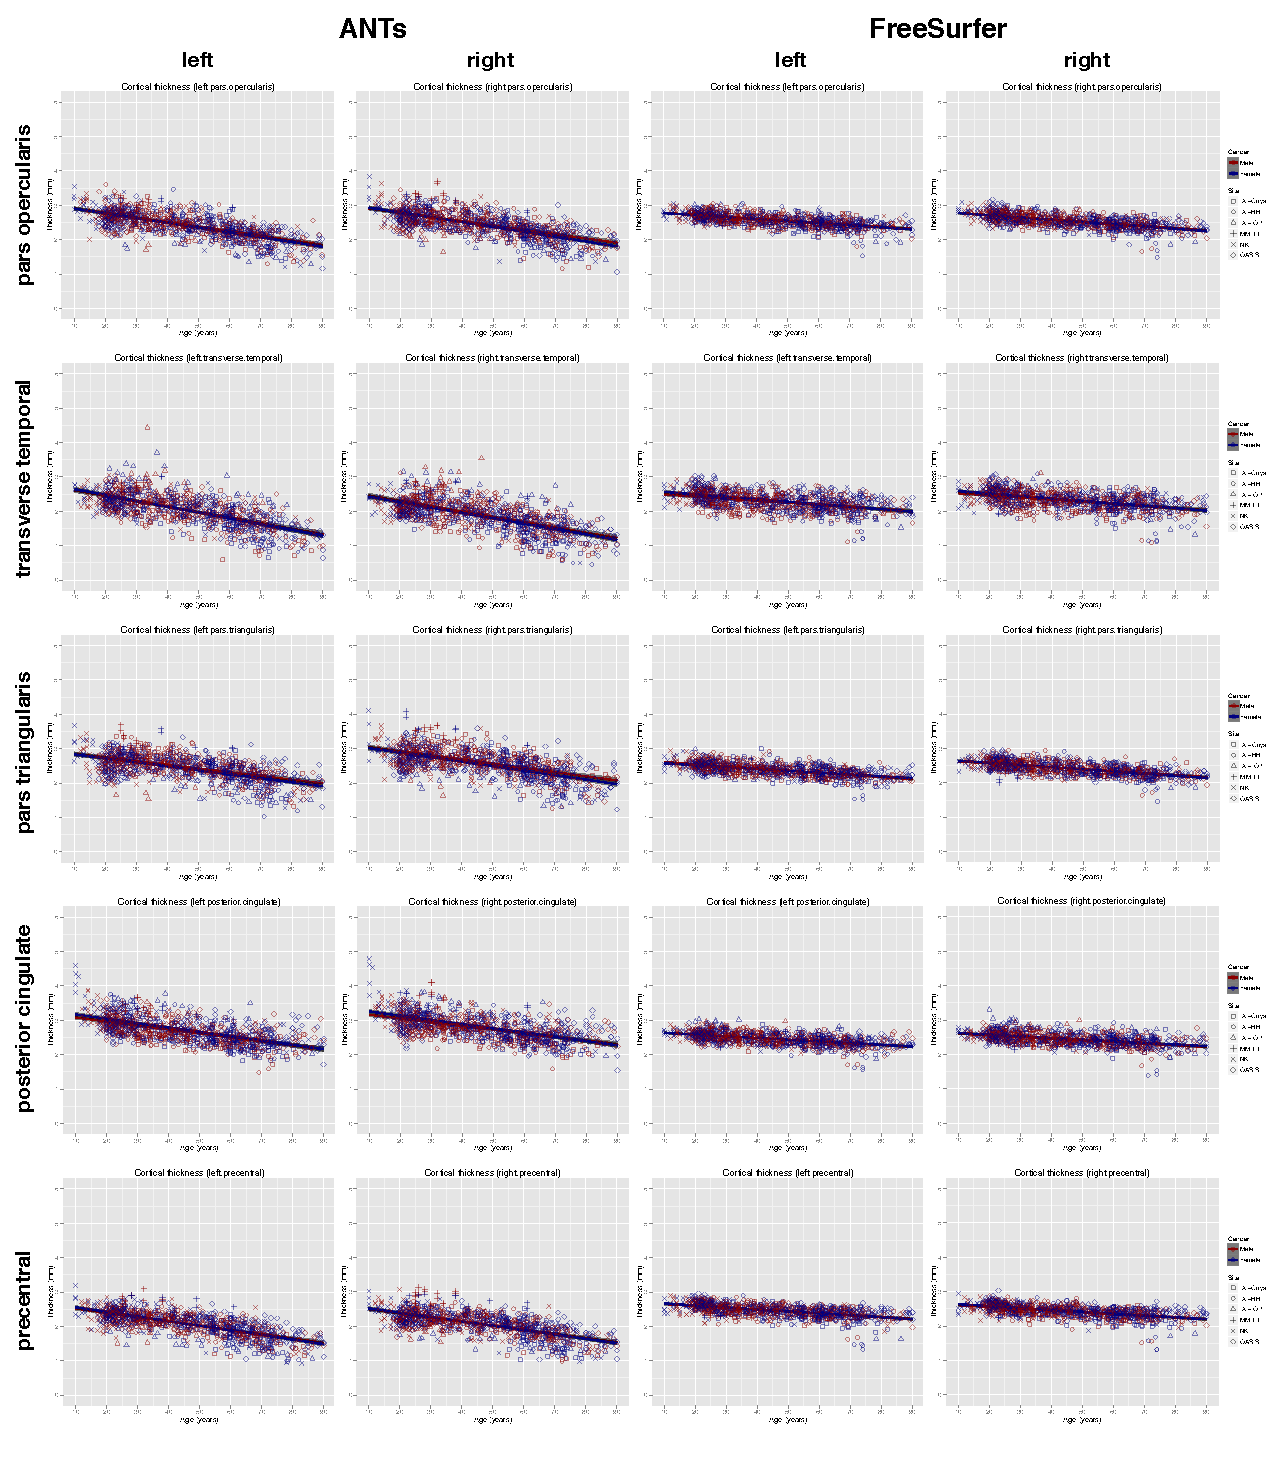
\includegraphics[width=0.99 \textwidth]{../Figures/rfImportanceRegions.pdf}

\end{frame}

\begin{frame}{Cross-sectional evaluation (age prediction)}

\centering
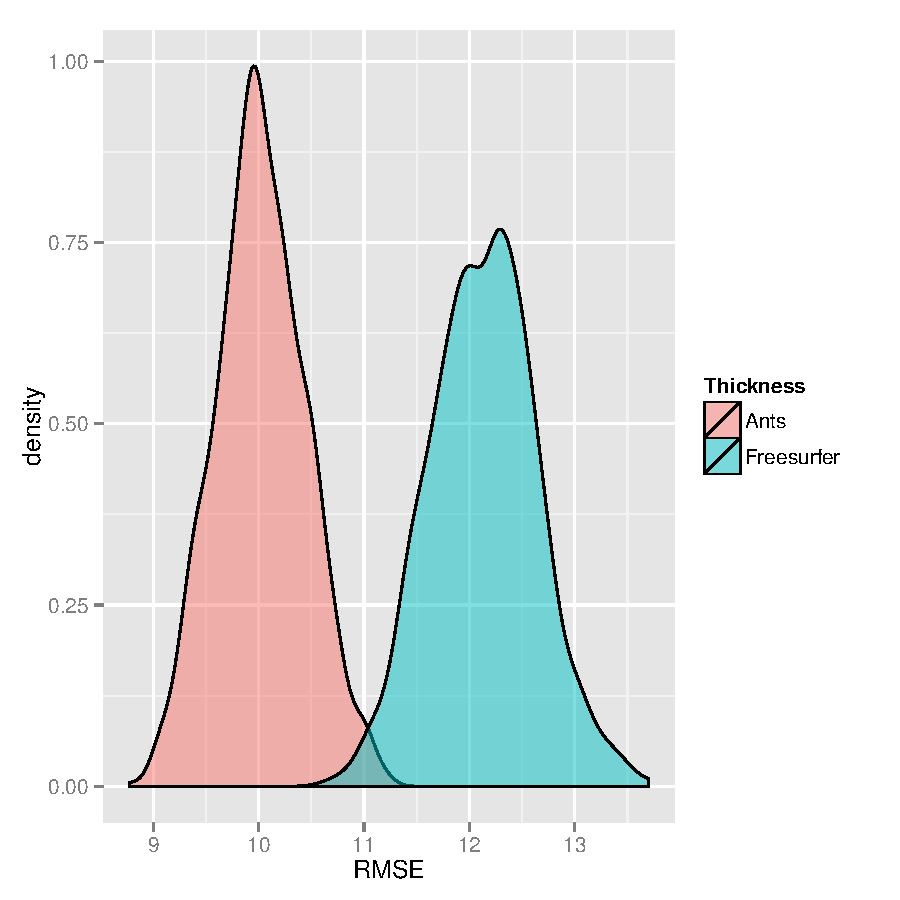
\includegraphics[width=0.5 \textwidth]{../Figures/rfRmse075.pdf}

Repeatability: \(ICC_{FS} = 0.97, ICC_{ANTs} = 0.98\)

\end{frame}

\begin{frame}{Longitudinal comparison (ADNI-1)}

\centering
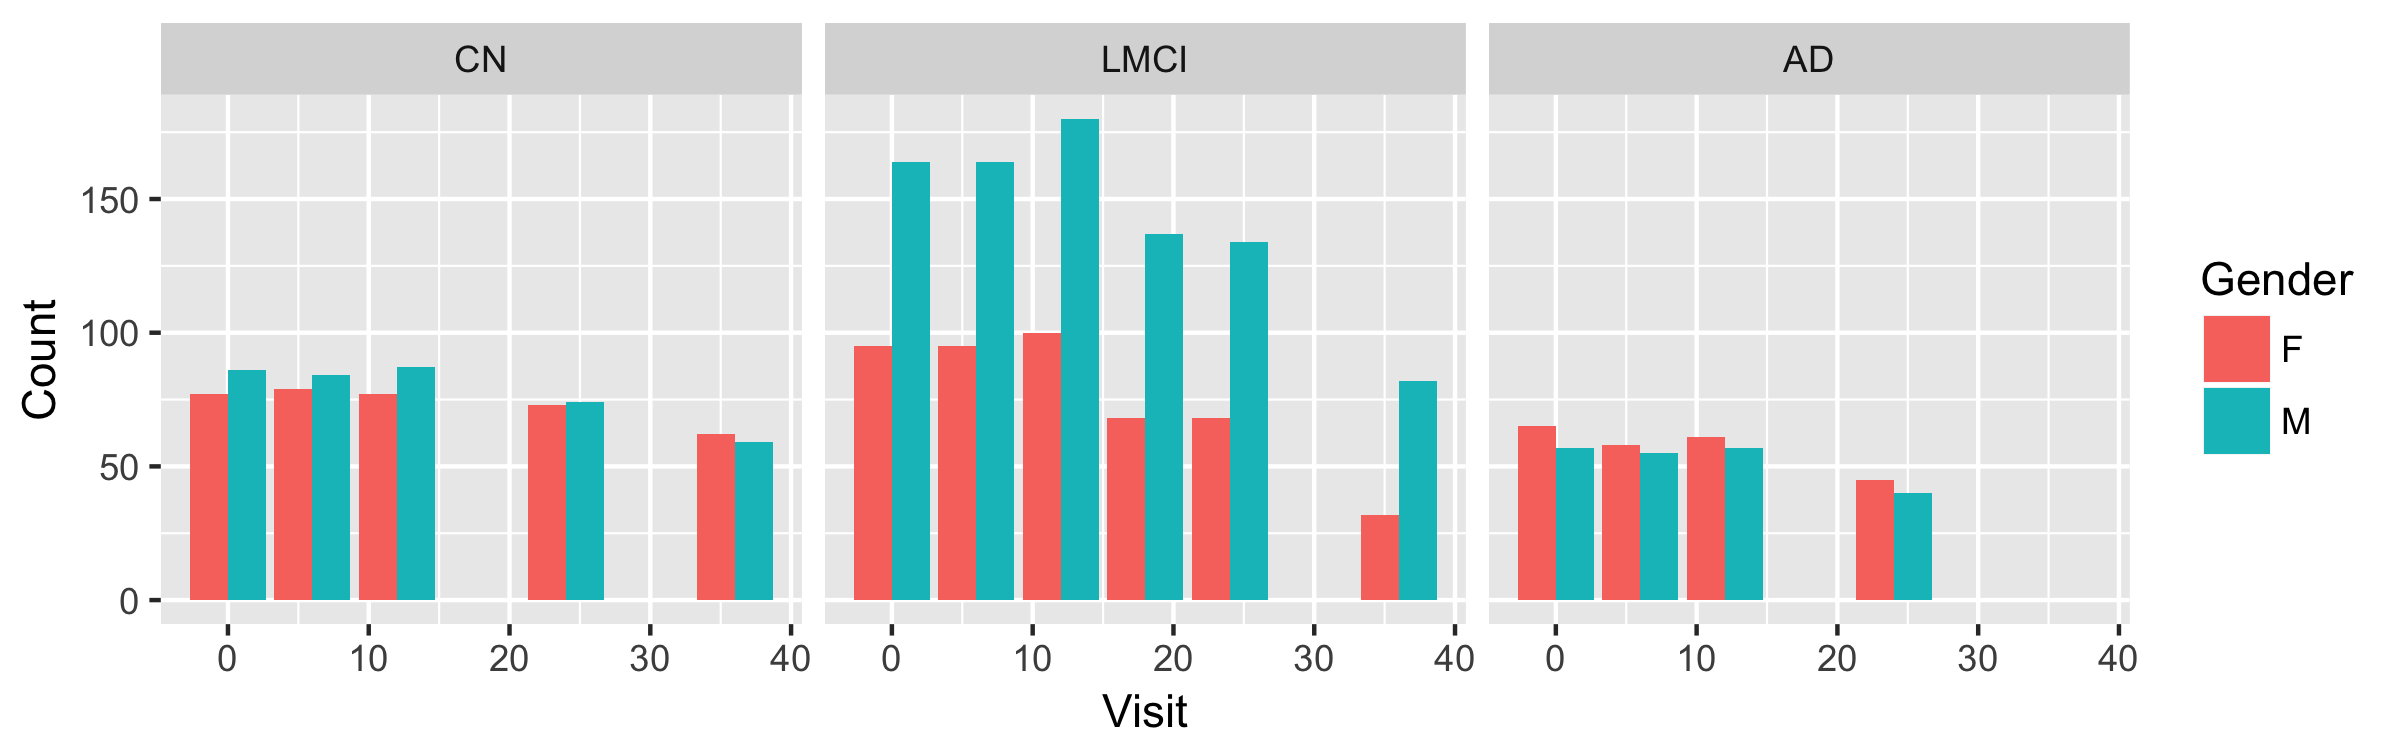
\includegraphics[width=0.99 \textwidth]{../Figures/demoPlot.png}

\end{frame}

\begin{frame}{Spaghetti plots (left insula)}

\centering
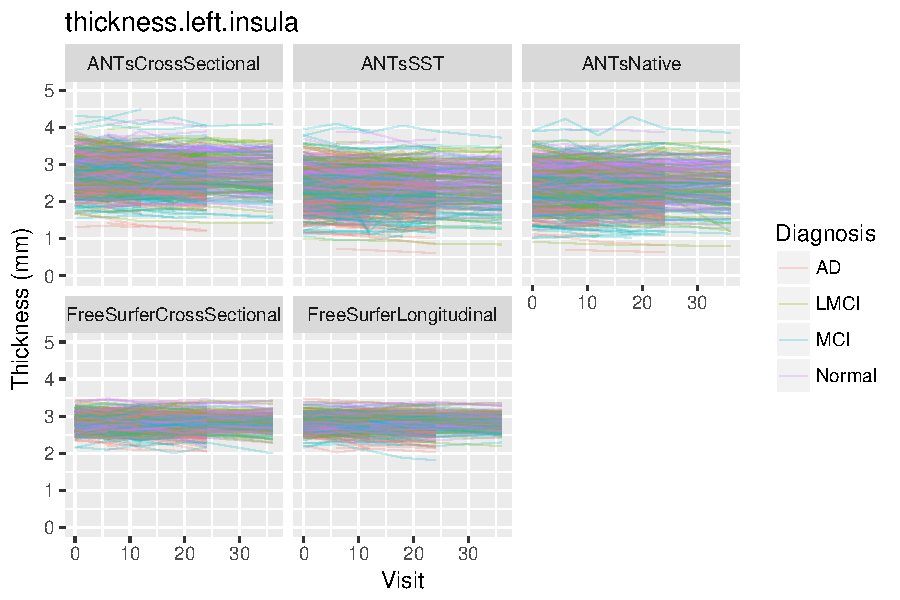
\includegraphics[width=0.9 \textwidth]{../data/RegionalThicknessSpaghettiPlots/thicknessleftinsula.pdf}

\end{frame}

\begin{frame}{Spaghetti plots (left middle temporal)}

\centering
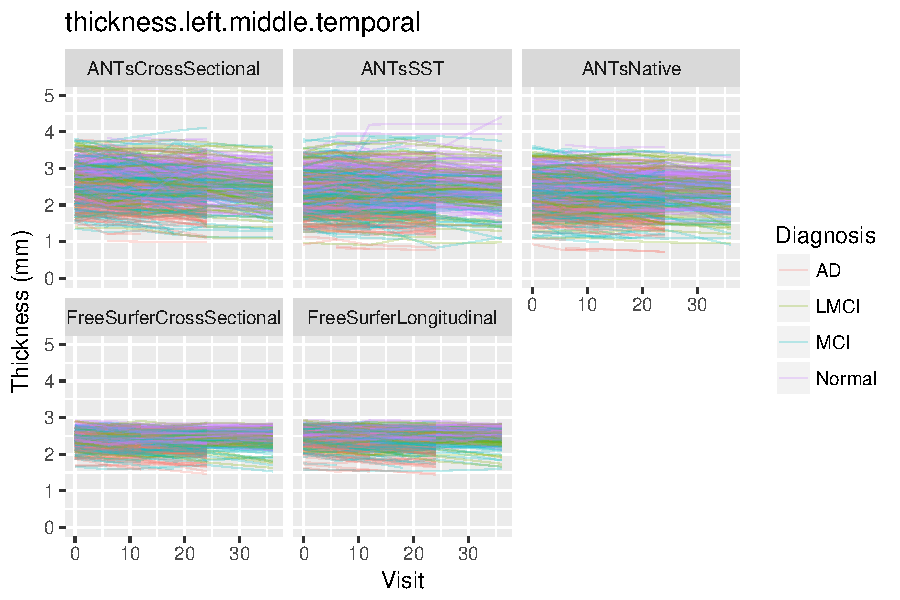
\includegraphics[width=0.99 \textwidth]{../data/RegionalThicknessSpaghettiPlots/thicknessleftmiddletemporal.pdf}

\end{frame}

\begin{frame}{Within-subject and between-subject variability}

\centering
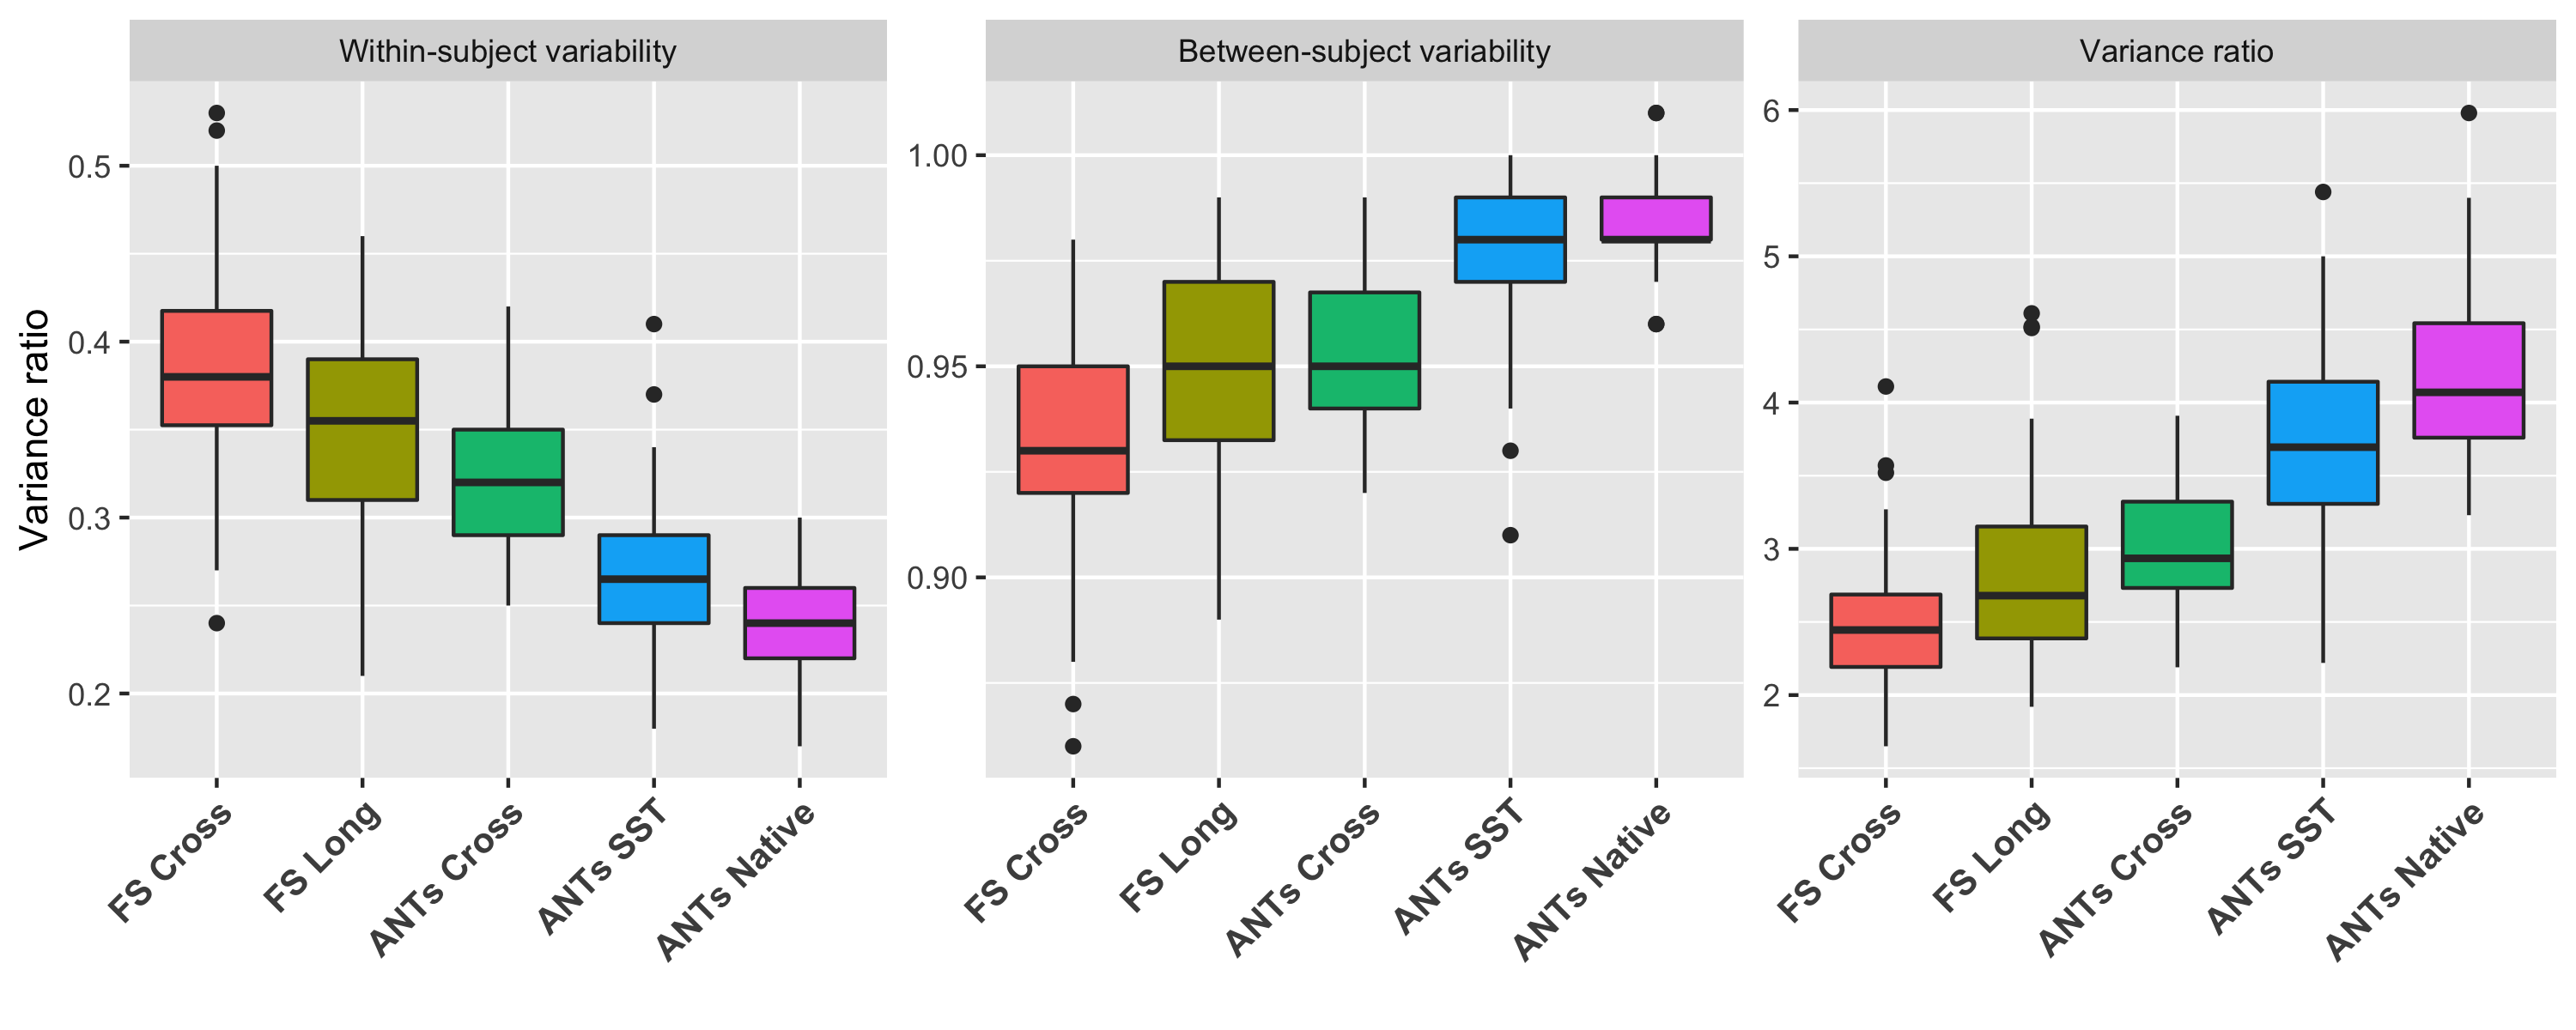
\includegraphics[width=0.99 \textwidth]{../Figures/allData_FINAL.png}

\end{frame}

\begin{frame}{Regional comparisons}

\centering
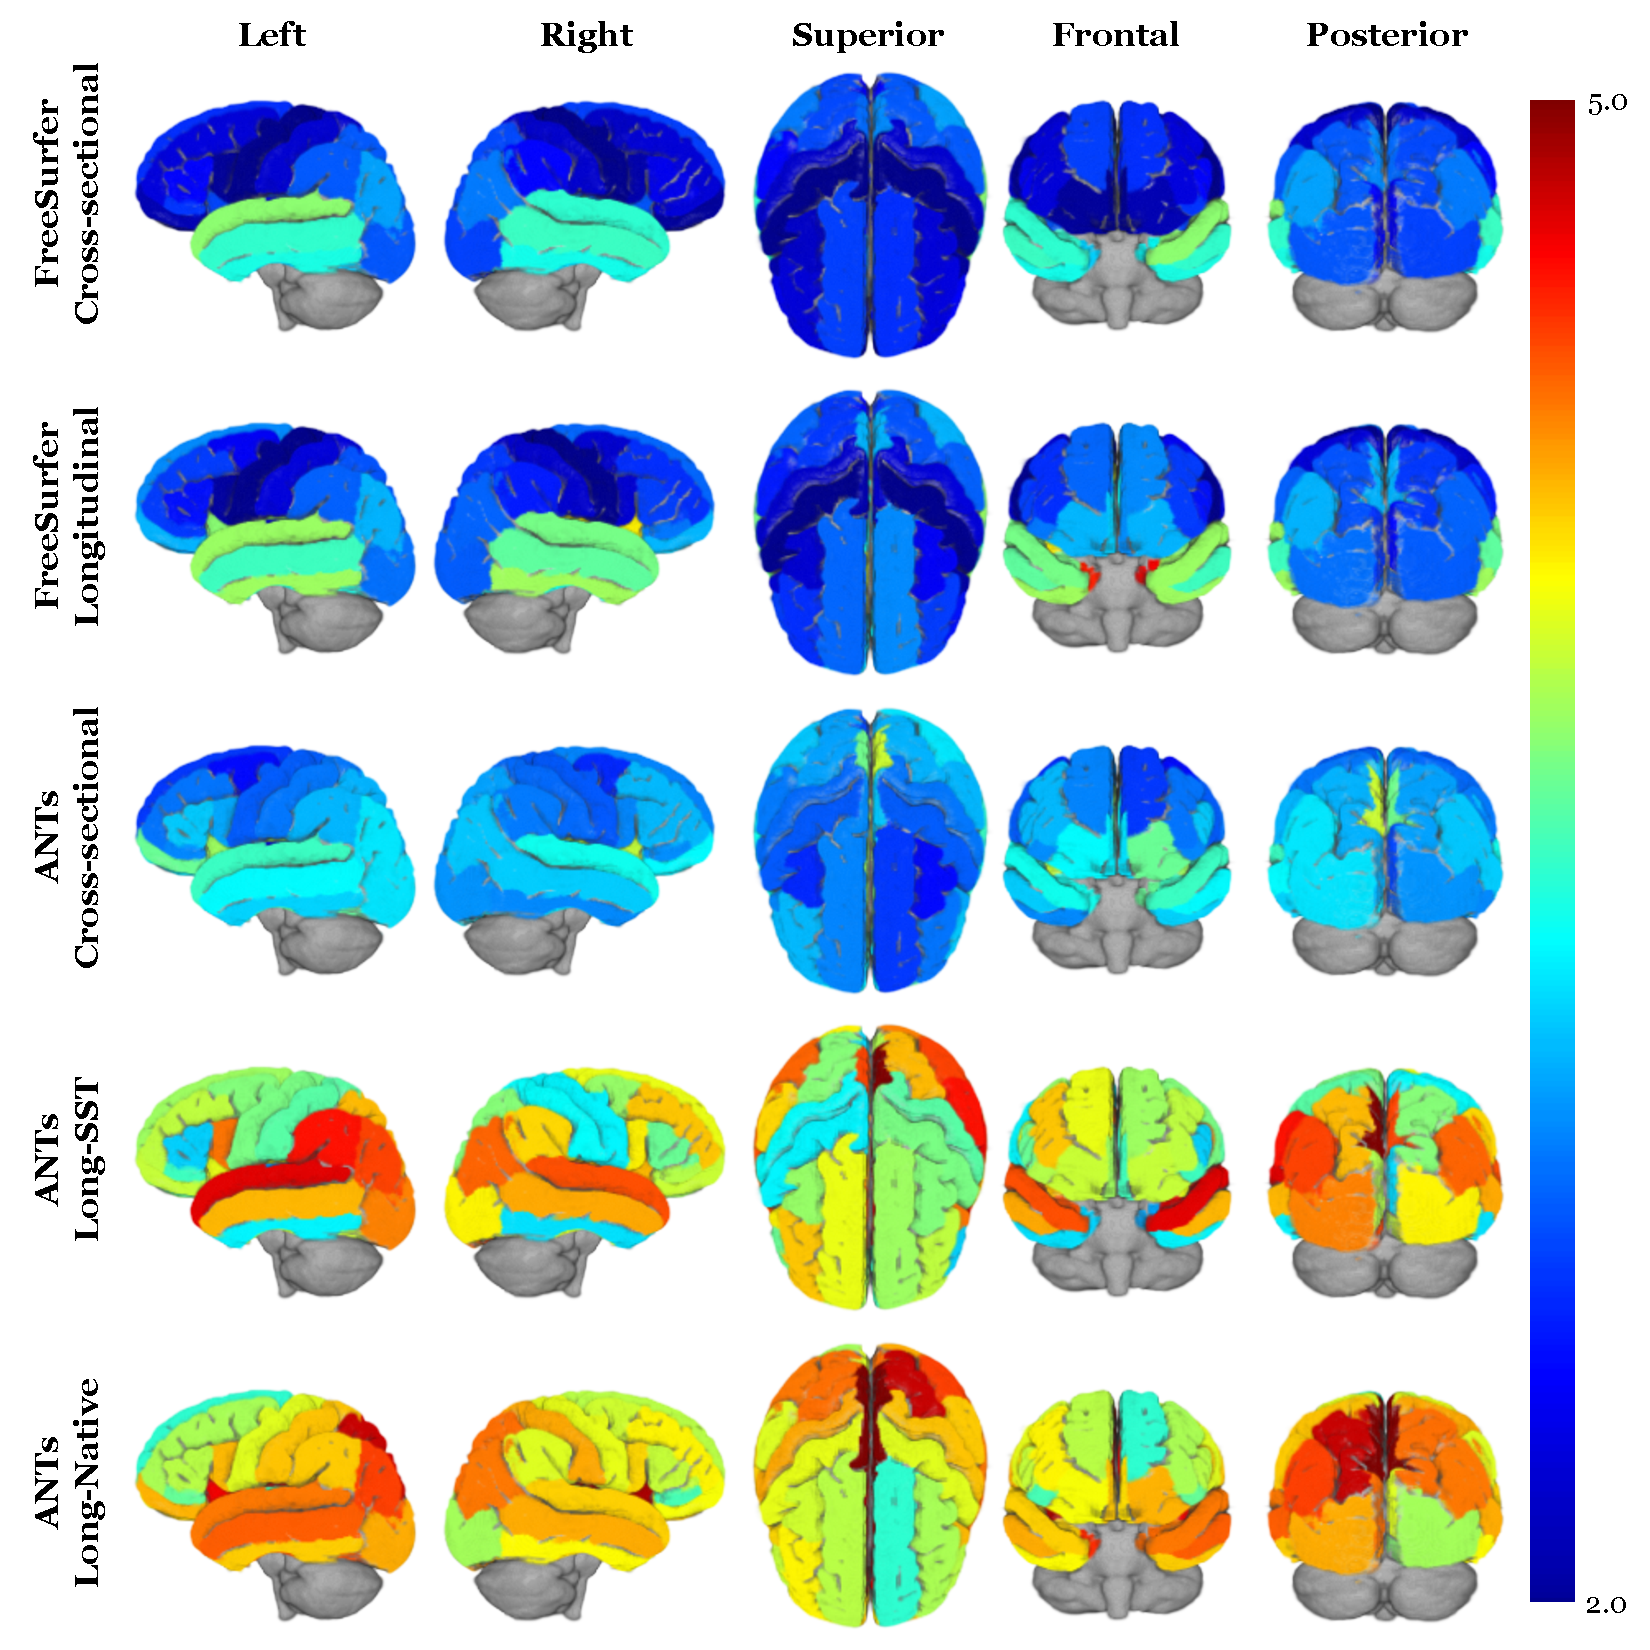
\includegraphics[width=0.65 \textwidth]{../Figures/medianRatios3D.pdf}

\end{frame}

\begin{frame}{Issues in the EC}

Xie et al., \emph{Accounting for the Confound of Meninges in Segmenting
Entorhinal and Perirhinal Cortices in T1-Weighted MRI}, MICCAI 2016.

\centering
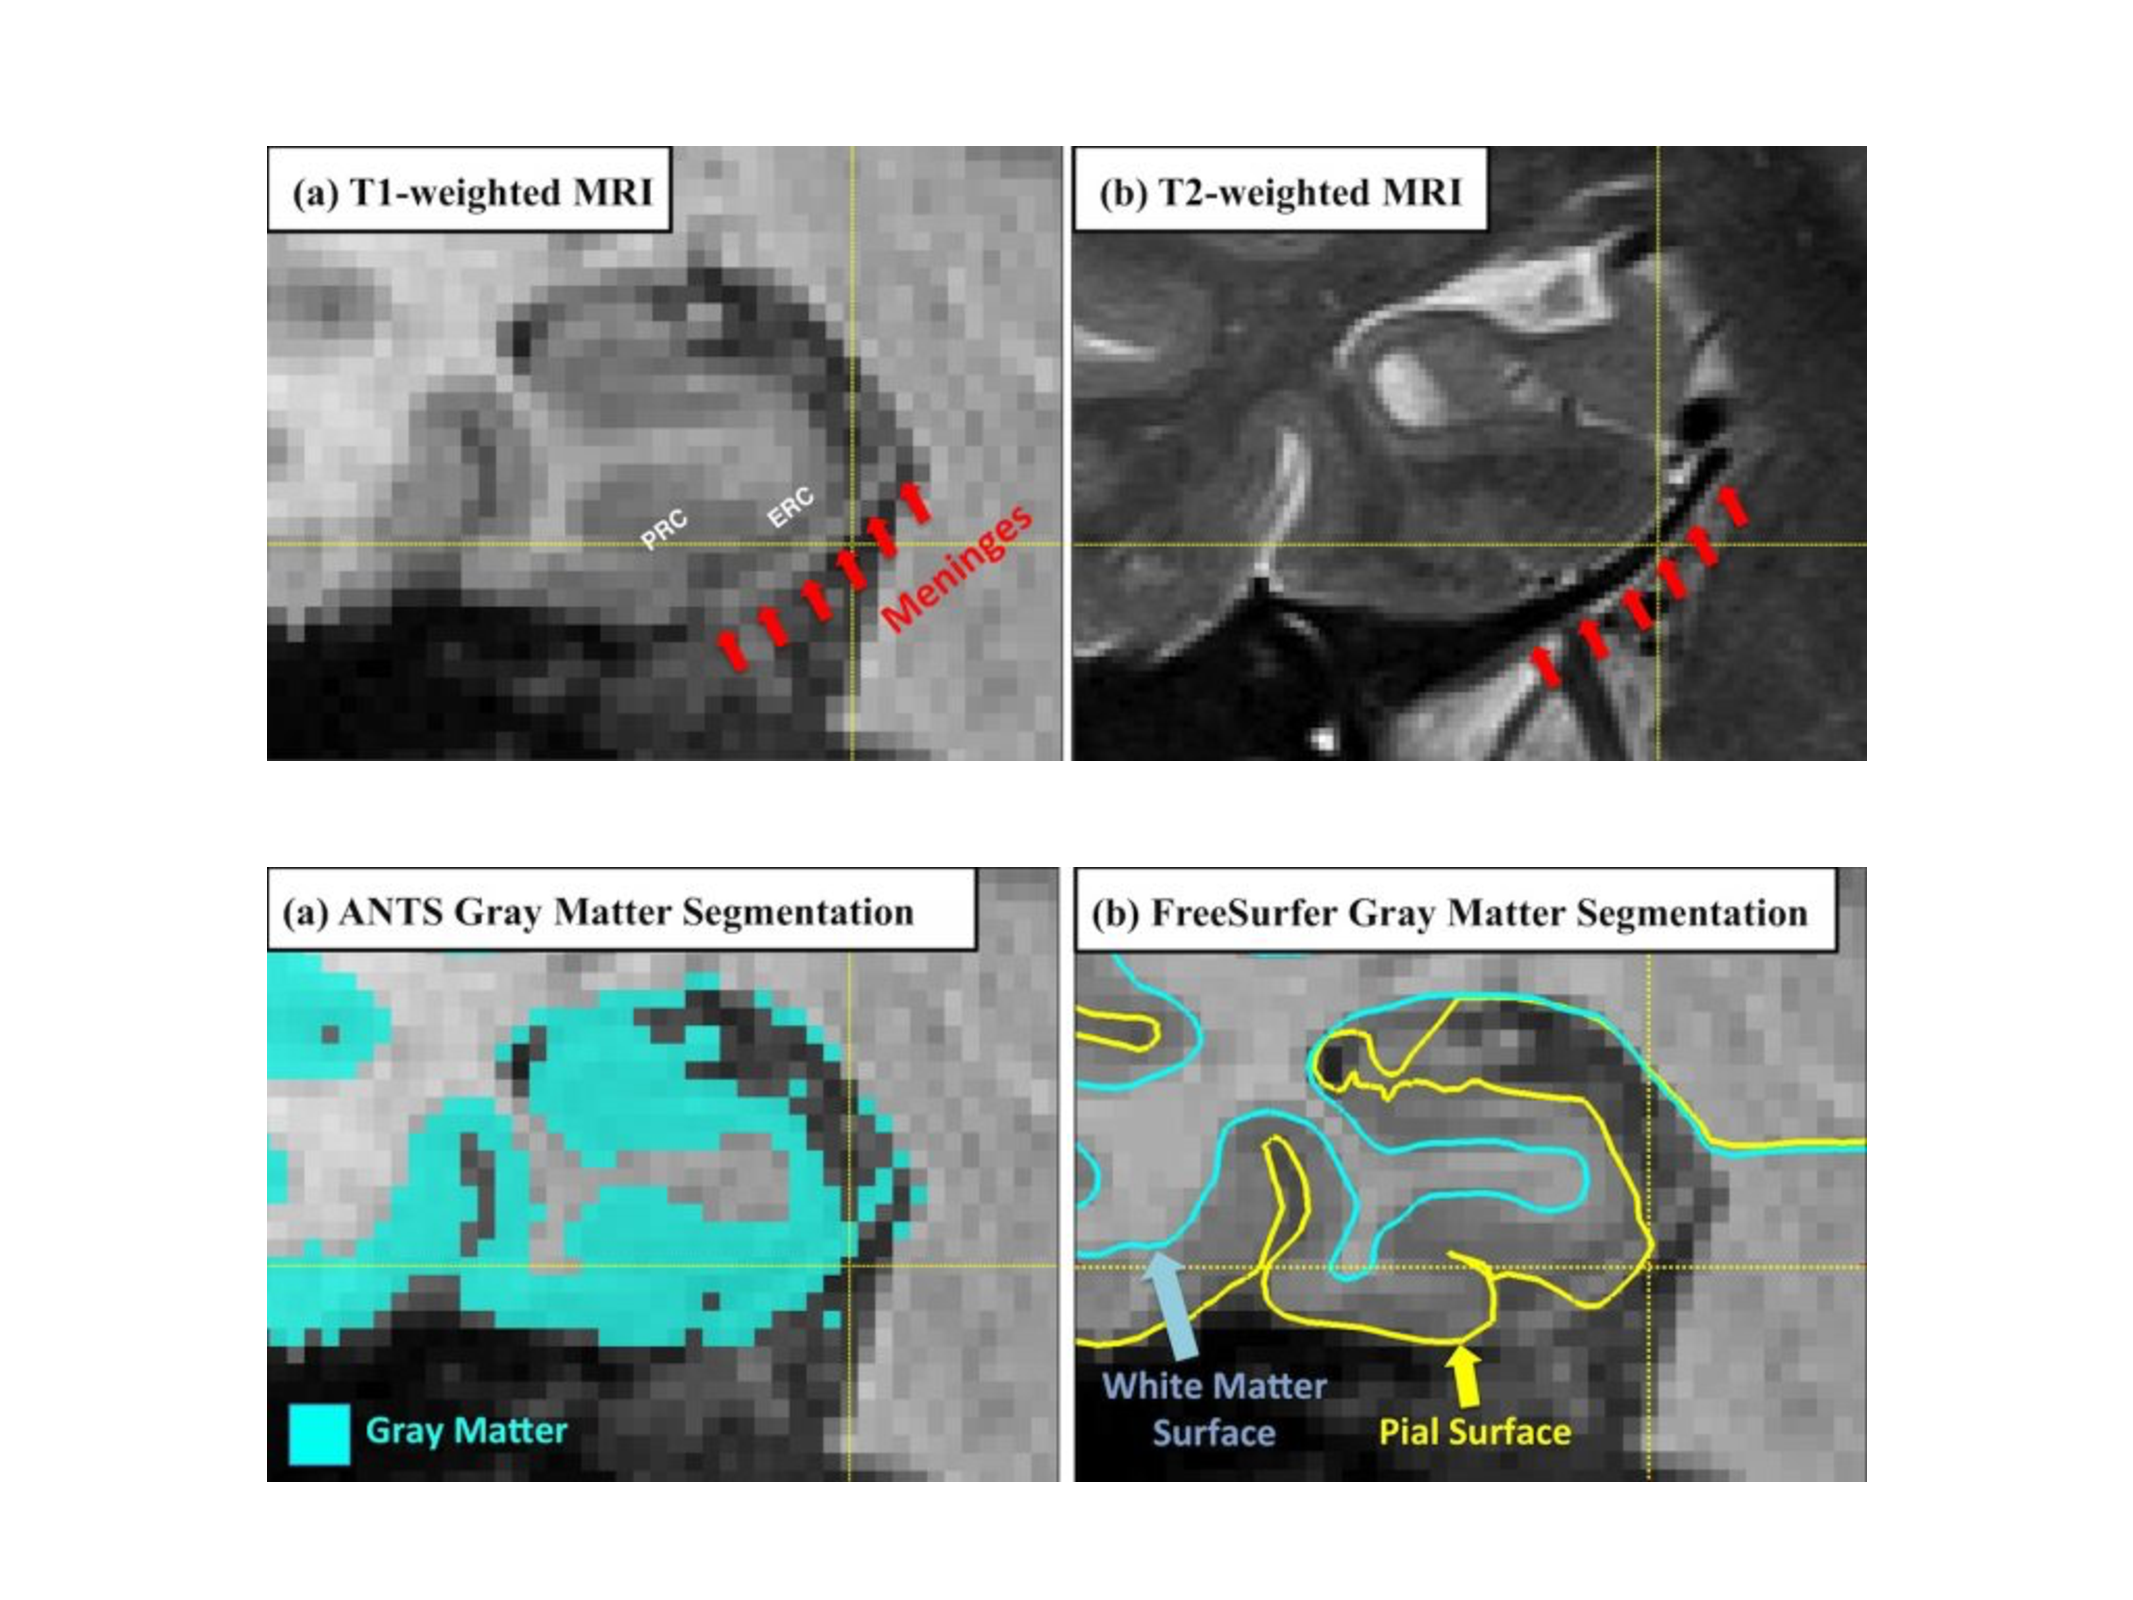
\includegraphics[width=0.7 \textwidth]{../Figures/LongXie.pdf}

\hypertarget{refs}{}

\end{frame}

\end{document}
